{ %section4_1
	\subsection{Порядок выполнения работы}
	\Large
	\begin{enumerate}
		\itemНа компьютере с многоядерным процессором установить ОС Linux и компилятор GCC версии не ниже 4.7.2. При невозможности установить Linux или отсутствии компьютера с многоядерным процессором можно выполнять лабораторную работу на виртуальной машине.
		\itemНа языке Cи написать консольную программу lab1.c, решающую задачу, указанную в п.IV (см. ниже). В программе нельзя использовать библиотечные функции сортировки, выполнения матричных операций и расчёта статистических величин. Задача должна решаться 100 раз с разными начальными значениями генератора случайных чисел (ГСЧ).  Структура программы примерно следующая:
			\begin{figure}[H]
				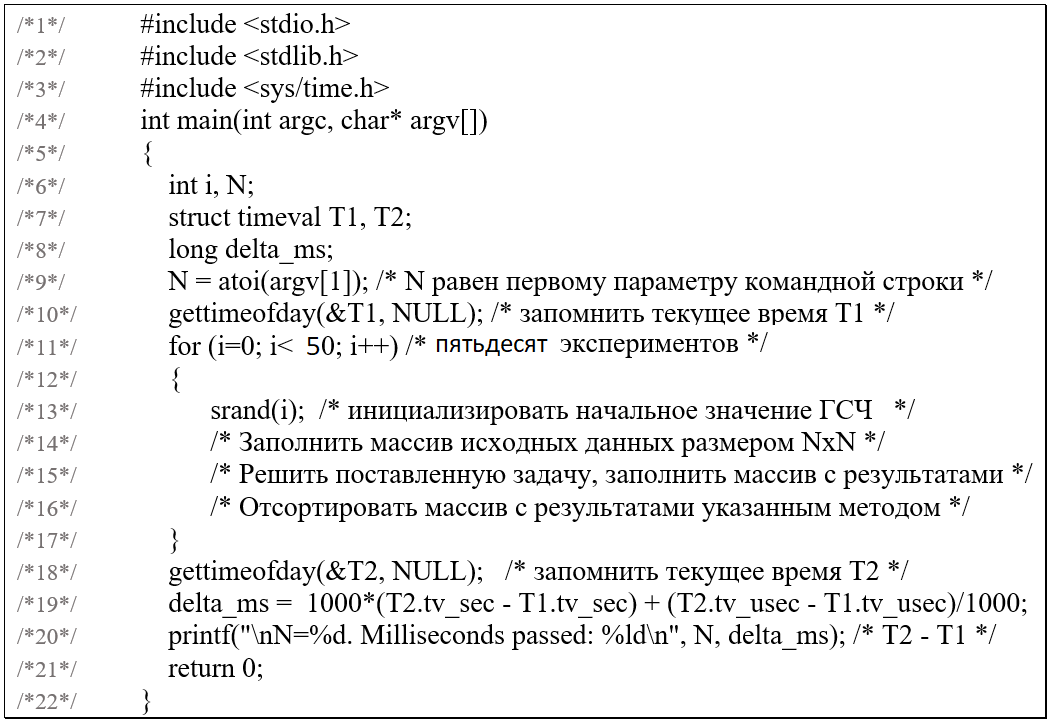
\includegraphics[width=1\linewidth]{lab1Example}
			\end{figure}
		\itemСкомпилировать написанную программу без использования автоматического распараллеливания с помощью следующей команды: /home/user/gcc -O2 -Wall -Werror -o lab1-seq lab1.c
		\itemСкомпилировать написанную программу, используя встроенное в gcc средство автоматического распараллеливания Graphite с помощью следующей команды “/home/user/gcc -O2 -Wall -Werror -floop-parallelize-all -ftree-parallelize-loops=K lab1.c -o lab1-par-K” (переменной K поочерёдно присвоить десять различных целых значений).
		\itemВ результате получится одна нераспараллеленная программа и десять распараллеленных.
		\itemЗакрыть все работающие в операционной системе прикладные программы (включая Winamp, uTorrent, браузеры и Skype), чтобы они не влияли на результаты последующих экспериментов.
		\itemЗапускать файл lab1-seq из командной строки, увеличивая значения N до значения N1, при котором время выполнения превысит 0.5 с. Подобным образом найти значение N=N2, при котором время выполнения превысит 100 с.
		\itemИспользуя найденные значения N1 и N2, выполнить следующие эксперименты (для автоматизации проведения экспериментов рекомендуется написать скрипт):
			\begin{itemize}
				\itemзапускать lab1-seq для значений \\$N\;=\;{N1,\;N1+\Delta,\;N1+2\Delta,\;N1+3\Delta,…,\;N2}$ и записывать получающиеся значения времени delta\textunderscore ms(N) в функцию seq(N);
				\itemзапускать lab1-par-K для значений \\$N\;=\;{N1,\;N1+\Delta,\;N1+2\Delta,\;N1+3\Delta,…,\;N2}$ и записывать получающиеся значения времени delta\textunderscore ms(N) в функцию par-K(N);
				\itemзначение $\Delta$ выбрать так: $\Delta\;=\;(N2\;-\;N1)/10$.
			\end{itemize}
		\itemНаписать отчёт о проделанной работе.
		\itemПодготовиться к устным вопросам на защите.
		\item*\quadИзучить документацию к библиотеке Graphite и изменить программу так, чтобы эффект от распараллеливания увеличился. Экспериментально выяснить, как именно нужно выбирать значения К для получения наибольшего ускорения. Это дополнительное необязательное задание «со звёздочкой» повышенной сложности.
	\end{enumerate}
	
}